\documentclass{article}
\usepackage{amsmath}
\usepackage{amsfonts}
\usepackage{amsthm}
\usepackage{amssymb}
\usepackage{enumitem}
\usepackage{graphicx}
\usepackage{dsfont}
\usepackage{subcaption}
\DeclareMathOperator{\E}{\mathbb{E}}
\DeclareMathOperator{\Bern}{Bern}
\DeclareMathOperator{\Pois}{Pois}
\DeclareMathOperator{\Var}{Var}
\DeclareMathOperator{\R}{\mathbb{R}}
\newtheorem{lemma}{Lemma}
\newtheorem{theorem}{Theorem}
\newtheorem{example}{Example}
\usepackage[utf8]{inputenc}

\title{Asymptotic behaviour on Hypothesis Testing }
\author{zhaof17 }
\date{May 2021}

\begin{document}

\maketitle

\section{Hypothesis Testing}
Consider the hypothesis testing problem,
\begin{equation}
    \begin{cases}
    H=0 & \textrm{(null)} \quad X \sim P \\
    H=1 & \textrm{(alternative)} \quad X \sim Q
    \end{cases}
\end{equation}
Given one sample $x$, we will decide a test
$\widehat{H}: \mathcal{X} \to \{0,1\}$.

The type I error is defined as $\pi_0 = P(\widehat{H}=1
| H=0)$, also called false positive or false alarm.

The type II error is defined as $\pi_1 = P(\widehat{H}=0
| H=1)$,
also called false negative or missing detection.

Let $A\triangleq \{x\in \mathcal{X}: \widehat{H}(x)=1\}$
be the accept region for $H=1$.
\begin{theorem}[Neyman-Pearson Lemma]\label{thm:np}
Let $A_{\gamma} = \{x:Q(x) > \gamma P(x)\}$
for $\gamma \in \R$ be the accept region for $H=1$. Then for any accept region $A'$,
if $\pi_1(A') < \pi_1(A_{\gamma})$,
then $\pi_0(A') > \pi_0(A_{\gamma})$.
\end{theorem}
$A_{\gamma}$ is equivalent to log-likelihood ratio
test.

For discrete $\mathcal{X}$, we have
\begin{equation}\label{eq:p0p1}
\pi_0 + \lambda \pi_1 \geq \lambda - \sum_{x\in \mathcal{X}} (P(x) - \lambda Q(x))^{-}
\end{equation}

Theorem \ref{thm:np} implies that
when $\pi_1$ decreases, $\pi_0$ increases.

If random decision rule is considered,
for all decisions, the reachable $\pi_0-\pi_1$ curve
has the following shape in Fig. \ref{fig:pi01}
\begin{figure}[!ht]
\begin{subfigure}{0.45\textwidth}
    \centering
    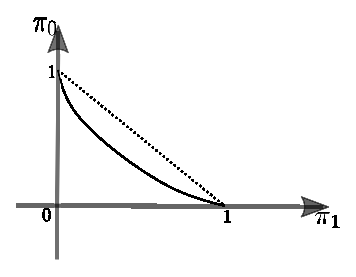
\includegraphics{pi0pi1.eps}
    \caption{$\pi_0-\pi_1$ curve}
    \label{fig:pi01}
\end{subfigure}~
\begin{subfigure}{0.45\textwidth}
    \centering
    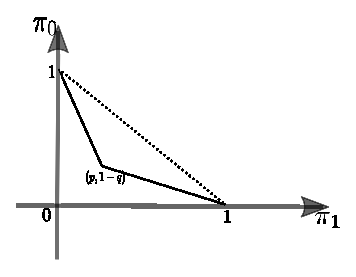
\includegraphics{pi0pi1_bern.eps}
    \caption{$\pi_0-\pi_1$ curve for Example \ref{ex:1}}
    \label{fig:pi01_bern}
\end{subfigure}
\caption{}
\end{figure}
The dotted line shows the random guess decision
rule. That is for the operating point $(1-p,p)$.
The decision rule is simply determined by a random number generated from $\Bern(p)$
regardless of the data distribution $P$ and $Q$.
The solid curve can be reached by LRT test. Points in the 
regions between the two curves are reachable
operating points, which perform better than random guess.
\begin{proof}[Proof of Theorem \ref{thm:np}]
We only need to  show that
\begin{equation}
\pi_0(A') + \gamma \pi_1(A')
\geq \pi_0(A_{\gamma}) + \gamma \pi_1(A_{\gamma})
\end{equation}
This is because
\begin{align*}
    \gamma \pi_0(A') + \pi_1(A')
    &= \gamma P(A') +Q(\bar{A}') \\
    &= \gamma\E_P[\mathds{1}_A(X)]
    + \E_Q[1-\mathds{1}_A(X)] \\
    &=1+ \gamma \E_P[\mathds{1}_A(X)]
    - \E_P[\frac{Q(x)}{P(x)}\mathds{1}_A(X)] \\
    &=1 + \E_P[\mathds{1}_A(X)(\gamma - \frac{Q(x)}{P(x)})]\\
    &\stackrel{(a)}{\geq} 1 + \E_P[\mathds{1}_{A'}(X)(\gamma - \frac{Q(x)}{P(x)})]\\
    &=\pi_0(A_{\gamma}) + \gamma \pi_1(A_{\gamma})
\end{align*}
where (a) holds since the set $A'$ is the maximal
set which minimizes $\sum_{x\in A} P(x)(\gamma - \frac{Q(x)}{P(x)})$.
\end{proof}
\begin{example}\label{ex:1}
Consider hypothesis testing between two
Bernoulli random variables, $P=\Bern(p), Q=\Bern(q)$
such that $p<\frac{1}{2}<q$. We can verify that
the solid curve in Fig. \ref{fig:pi01} becomes
a piece-wise linear line with turning point $(p,1-q)$.
\end{example}
In the above example, we emphasize that only
end point $(0,1),(1,0),(p,1-q)$ are achievable
for deterministic test. For a large domain of
$\gamma$, the error configuration is fixed
at $(p, 1-q)$.
Other points on the
solid lines are achieved by introducing
random decision rule: when $\widehat{H}(x)=1$, with probability $p'$ accept $H=1$ and
with probability $1-p'$ accept $H=0$. By
varying the extra parameter $p'$ we can obtain
points on solid lines.
\section{Multiple samples}
In this section we consider the two types of error
when multiple samples are observed.
Let $x^n = (x_1, \dots, x_n)$ be i.i.d. sampled from either
$P$ or $Q$.
\begin{equation}
    \begin{cases}
    H=0 & \textrm{(null)} \quad X^n \sim P^n \\
    H=1 & \textrm{(alternative)} \quad X^n \sim Q^n
    \end{cases}
\end{equation}
where $P^n$ or $Q^n$ represents the joint distribution of distribution of $X^n$. Then the LRT is rewritten
as $\frac{1}{n}\sum_{i=1}^n \ell(x_i)$ where
$\ell(x)=\log \frac{Q(x)}{P(x)}$. The decision rule for LRT
is
\begin{equation}\label{eq:AgammaN}
    A_{\gamma} \triangleq \{
x^n: \frac{1}{n}\sum_{i=1}^n \ell(x_i) > \gamma
\}
\end{equation}
and the two types of error are given by
\begin{align*}
    \pi_0^{(n)} &= P^n(A_{\gamma}) \\
    \pi_1^{(n)} &= Q^n(\bar{A}_{\gamma})
\end{align*}
For given $\gamma$, we first analyze the decaying
rate of $\pi_0^{(n)}$ and $\pi_1^{(n)}$.
We define the decay exponent as
\begin{equation}
    E_i \triangleq -\lim_{n\to \infty} \frac{1}{n}
    \log \pi_i^{(n)}\textrm{ for } i=0,1
\end{equation}
Then $\pi_0^{(n)} \doteq \exp(-n E_0)$
and $\pi_1^{(n)} \doteq \exp(-n E_1)$.
\subsection{Analysis of exponent with Cramér's Theorem}
The analysis is based on the Cramér's Theorem
and is applied to the sample mean of $\ell(x_i)$.
To make both two types of error decay, we should require
$\gamma$ lies in between $(-D(P||Q), D(Q||P))$. The end point
be obtained by computing $\E_P[l(X)]$ and $\E_Q[l(X)]$ directly. $\gamma = -D(P||Q)$ implies $\pi_0^{(n)}\to 1$
while $\gamma = D(Q||P)$ implies $\pi_1^{(n)}\to 1$.

For the non-trivial case, that is, $-D(P||Q) < \gamma < D(Q||P)$, we can quickly obtain that
$E_0 = \psi^*_P(\gamma)$ and $E_1 = \psi^*_Q(\gamma)$.

Let the log-MGF $\psi_P(\lambda)\triangleq \log \E_{P}
[\exp(\lambda \ell(X))] = \log \sum_{x\in\mathcal{X}}
[P(x)]^{1-\lambda}[Q(x)]^{\lambda}$.
Using $Q(x)=P(x)e^{\ell(x)}$, we can obtain
$\psi_Q(\lambda)\triangleq \log \E_{Q}
[\exp(\lambda \ell(X))] = \log \E_{P}
[\exp((\lambda +1)\ell(X))] = \psi_P(\lambda + 1)$.
Then
$\psi_P^*(\gamma)\triangleq \sup_{\lambda \in \R} [\lambda \gamma - \psi_P(\lambda)]$.
The optimal $\lambda$ is chosen to satisfy
$\psi_P'(\lambda) = \gamma$.
The relation can be rewritten as
$\psi_P'(\lambda) = \frac{\E_{P}
[\ell(X)\exp(\lambda \ell(X))]}{\E_{P}
[\exp(\lambda \ell(X))]}
=\E_{P}
[\ell(X)\exp(\lambda \ell(X)-\psi_P(\lambda))]
=\E_{P^{(\lambda)}}[\ell(X)]$ where the geometric mixture distribution
$P^{(\lambda)}$ is defined as 
\begin{equation}\label{eq:plambda}
    P^{(\lambda)}(x) = P(x)\exp(\lambda \ell(X)-\psi_P(\lambda))
    = \frac{
[P(X)]^{1-\lambda}[Q(x)]^{\lambda}
}{\sum_{x\in\mathcal{X}}
[P(X)]^{1-\lambda}[Q(x)]^{\lambda}}
\end{equation}
When $\lambda = 0$, $P^{(\lambda)} = P$ and $\gamma = -D(P||Q)$;
When $\lambda = 1$, $P^{(\lambda)} = Q$ and $\gamma = D(Q||P)$.
Besides, $\gamma$ is an monotonically increasing function of
$\lambda$ from the property of the conjugate log-MGF.
Therefore, the domain of definition for $\lambda$ is $(0,1)$ to guarantee $-D(P||Q) < \gamma < D(Q||P)$.

$\psi_Q^*(\gamma)$ can be expressed in term of
$\psi_P^*(\gamma)$:
$\psi_Q^*(\gamma)
=\sup_{\lambda \in \R} [\lambda \gamma - \psi_P(\lambda+1)]
=\psi_P^*(\gamma)-\gamma
$.

We can draw the function $\psi_P(\lambda)$ and illustrate it
in Fig. \ref{fig:psiell}. At the point $(\lambda_0, \psi_P(\lambda))$,
the slope of the tangent line is $\gamma$ such that
$\psi'_P(\lambda_0)=\gamma$. Since $\psi_P^*(\gamma) = \gamma \lambda_0 - \psi_P(\lambda_0)$. The geometric meaning of $E_0$ is the length
of the intercept for the tangent line, and $E_1$ is the length of
y-axis of the intersection between the tangent line and $\lambda=1$.
Fig. \ref{fig:psiell} also shows a right trapezoid whose
two bases have length $E_0$ and $E_1$. the lateral side
has length 1 on the right angle side. Finally, Fig.
\ref{fig:psiell} shows the trade-off between $E_0$ and $E_1$.
One error increases while the other decreases.
\begin{figure}[!ht]
    \centering
    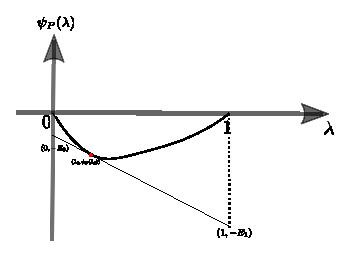
\includegraphics[width=0.6\textwidth]{e0e1.eps}
    \caption{log-MGF of $\ell(X)$}
    \label{fig:psiell}
\end{figure}

We summarize important formulas in this subsection:
\begin{align}\label{eq:cramer_important}
    \psi_P(\lambda)&=\log \sum_{x\in\mathcal{X}}
[P(x)]^{1-\lambda}[Q(x)]^{\lambda} \\
    \gamma &= \psi'_P(\lambda)= \frac{\sum_{x\in\mathcal{X}}
\log\frac{Q(x)}{P(x)}\cdot[P(X)]^{1-\lambda}[Q(x)]^{\lambda}}
{\sum_{x\in\mathcal{X}}
[P(X)]^{1-\lambda}[Q(x)]^{\lambda}} \\
E_0 &= \lambda \gamma - \psi_P(\lambda) \\
E_1 & = E_0 - \gamma
\end{align}
\subsection{Analysis of exponent with Sanov's Theorem}
Since we consider discrete random variables, Sanov's theorem
can be applied to obtain another illustration for $E_0$
and $E_1$.
That is $E_0 = \min_{R\in \mathcal{L}_{\gamma}}D(R || P)$ and $E_1=\min_{R\in \mathcal{L}_{\gamma}}D(R ||Q)$ where
$R$ is the empirical distribution on the hyper-plane
$\mathcal{L}_{\gamma}\triangleq\{R: \E_R[\ell(X)]=\gamma \}$.
We use $L_{\gamma}^+$ to represent the space when
$\E_R[\ell(X)]>\gamma$. $L_{\gamma}^-$
is defined similarly.
By Lagrange's method, we can find a distribution $P^{(\lambda)}$
defined in \eqref{eq:plambda} and belongs to $\mathcal{L}_{\gamma}$.
As we change $\gamma$ from $-D(P||Q)$ to $D(Q||P)$, $\lambda$ changes
from $0$ to $1$, and the distribution $P^{(\lambda)}$ changes from
$P$ to $Q$. the change path for $P^{(\lambda)}$ can be draw in
distribution space as shown in Fig. \ref{fig:ds}.
Then the two error exponents are the distances
$E_0 = D(P^{(\lambda)} || P)$ and $E_1=D(P^{(\lambda)} ||Q)$.
\begin{figure}
    \centering
    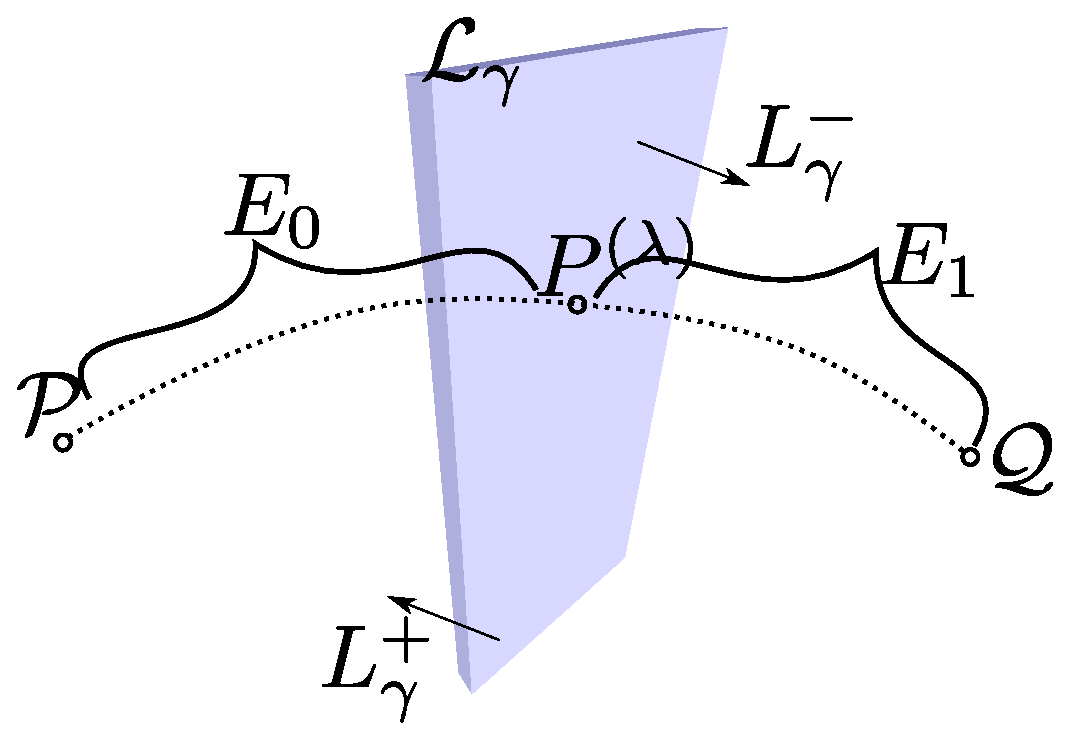
\includegraphics[width=0.7\textwidth]{distributional_space.eps}
    \caption{$E_0, E_1$ representation in distribution space}
    \label{fig:ds}
\end{figure}

There are two ways to study the optimal decay rate of $\pi_0^{(n)}$
and $\pi_1^{(n)}$. One way is calculating the fast exponential rate
of one error while controlling the other error within a given threshold. Or we try to minimize the weighted sum of the
two types of error
under Bayesian setting.
The first way is quantified by Chernoff-Stein Lemma, while the second is studied by Chernoff information.
\begin{theorem}[Chernoff-Stein Lemma]\label{thm:csl}
Let $\pi_0^{(n)} < \epsilon$,
and the optimal type II error $\hat{\pi}_1^{(n)}$
is defined as
$$
\hat{\pi}_1^{(n)} \triangleq \min_{A: \pi_0^{(n)}(A)<\epsilon}\pi_1^{(n)} (A)
$$.
Then $\lim_{n\to\infty} \frac{1}{n} \log \hat{\pi}_1^{(n)}
= -D(P||Q)
$.
\end{theorem}
From N-P Lemma, we should choose LLR test to achieve the 
minimal $\hat{\pi}_1^{(n)}$. If $E_0>0$, when $n$ is sufficiently
large, we have $\pi_0^{(n)} < \epsilon$.
Then from the analysis of the last
section, when we let $E_0 > 0$ to be arbitrarily small, we can
achieve $E_1$ arbitrarily close to $D(P||Q)$. That is,
we have $D(P||Q) \leq E_1 < D(P||Q) - \delta$ for any $\delta > 0$.
\begin{theorem}[Chernoff Information]
Consider the error probability defined as
$P_e^{(n)}=P(\widehat{H}\neq H)
=P(\widehat{H}=1)\pi^{(n)}_0
+P(\widehat{H}=0)\pi^{(n)}_1$. Then
\begin{equation}\label{eq:minPe}
    \inf \liminf_{n\to\infty}
    \frac{1}{n} \log P_e^{(n)}
    = - \psi_P^*(0)
\end{equation}
where $\psi_P^*(0)=-\min_{\lambda \in [0,1]}
\log \sum_{x\in \mathcal{X}}[P(X)]^{1-\lambda}[Q(x)]^{\lambda}
$
\end{theorem}
Notice that $\psi_P^*(0)$ corresponds to $\gamma=0$,
which means the slope equals to zero in Fig.
\ref{fig:ds}. This limit is achieved for LRT
with $\lambda$ satisfying $\psi'_P(\lambda)=0$.
In such case, $E_0=E_1=\psi_P^*(0)$.
For the error of other detection
method, $P_e^{(n)}\doteq \exp(-n \min\{E_0, E_1\})$.
By NP Lemma, when adopting decision rules other than
LRT, $\min\{E_0, E_1\}$ will become smaller. Thus
left hand side in \eqref{eq:minPe} becomes
larger. As a result, we only need to consider
LRT, that is, to maximize $\min\{E_0, E_1\}$.
From Fig.
\ref{fig:ds}, the maximization is achieved
when $\gamma=\psi'_P(\lambda)=0$.
\begin{example}\label{ex:2}
We extend Example \ref{ex:1} and consider
$n$ samples either from $\Bern(p)$ or $\Bern(q)$.
NP-Test has the following form (from \eqref{eq:AgammaN}):
\begin{equation}
A_{\gamma}: \frac{x_1 + \dots + x_n}{n} > \tilde{\gamma} \textrm{ where } \tilde{\gamma}
= \frac{\gamma - \log \frac{1-q}{1-p} }{\log \frac{q(1-p)}{p(1-q)}}
\end{equation}
For $n=2$, we describe the relationship
of $\pi_0, \pi_1$ in Figure \ref{fig:pi0n2}. Notice
that the solid line (representing $n=2$) is strictly
under the dotted line (representing $n=1$). The solid
line has two turning points (in red). As we increase $n$,
the $\pi_0-\pi_1$ curve becomes much closer to
the axes.
\end{example}
\begin{figure}[!ht]
    \centering
    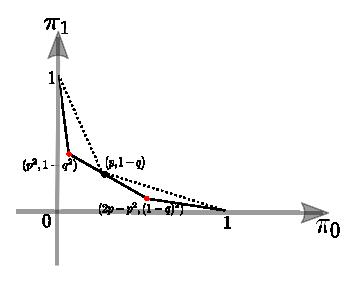
\includegraphics[width=0.6\textwidth]{pi0pi1_bern_2.eps}
    \caption{$\pi_0-\pi_1$ curve for $n=1,2$}
    \label{fig:pi0n2}
\end{figure}
We take $p=0.3,q=0.8$ in Example
\ref{ex:2}, and compute $E_0, E_1$ for
$\lambda \in (0,1)$ from series of formulas in 
\eqref{eq:cramer_important}. The result is shown
in Figure \ref{fig:trade}
\begin{figure}[!ht]
    \centering
    \includegraphics[width=0.6\textwidth]{trade_off.eps}
    \caption{}\label{fig:trade}
\end{figure}
We make a few remarks.
\begin{enumerate}
    \item $E_1$ is a decreasing function of $E_0$;
    \item $\max E_1 = D(P||Q)$ and $\max E_0 = D(Q||P)$,
    which are error exponent achieved in Chernoff-Stein Lemma;
    \item The Chernoff information is the intersection
    of $E_1=E_0$ with the curve.
\end{enumerate}
\section{Type-based test}
 We say a test
 is optimal among all tests whose exponent $E_0 \geq \eta$, it has the largest $E_1$ exponent.
 Notice that the optimality of a test is studies
 in asymptotic region.
 In this section, we want to answer the following
 three questions based on Theorem
 \ref{thm:type_based} and Theorem.
 \begin{enumerate}
     \item Is NP-Test the only optimal test? (No, we have generalized likelihood ratio test)
     \item Is type-based decision (test) optimal?
     (Yes, when we consider optimal test, we only need to consider the decision rule which is
     functions of empirical measure of the data)
     \item Are both underlying distributions needed to construct an optimal test? (No, we only need
     distribution $P$.)
 \end{enumerate}
 For the third question, we notice that NP-Test
 in the form of \eqref{eq:AgammaN}
 depends on both underlying distribution $P$
 and $Q$.
 
 Firstly we give a theorem that answers the second question, that is, given any test, we can construct
 a type-based test whose errors are controlled by
 those of the given test.
\begin{theorem}\label{thm:type_based}
Given $\widehat{H}:
\mathcal{X}: \mathcal{X}^n \to \{0,1\}$, we can construct
a type-based decision $\widehat{H}':
\mathcal{X}^n \to \{0,1\}$ such that
$\pi_i(\widehat{H}') \leq 2\pi_i(\widehat{H}) $.
\end{theorem}
\begin{proof}
Let $A_1 \triangleq \{ x^n \in \mathcal{X}^n
: \widehat{H}(x^n) = 1 \}$. We define
\begin{equation*}
\widehat{H}'(x^n)
= \begin{cases}
1 & \textrm{ if }  \frac{|T_{\hat{P}_{X^n}} \cap A_1|}{|T_{\hat{P}_{X^n}}|} > \frac{1}{2}\\
0 & \textrm{ otherwise}
\end{cases}
\end{equation*}
where $T_{\hat{P}_{X^n}} $ is the type class of $x^n$. $\widehat{H}$ is actually a function of 
type class $Q_X$.

Suppose $Q_X$ is a type class satisfying $\widehat{H}'(Q_X)=1$.
Then $
\frac{P(\widehat{H}(Q_X)=1 | H=i)}{P(Q_X | H=i)}
= P(\widehat{H}(Q_X)=1 | Q_X, H = i)$ for $i=0,1$.
Given $Q_X$, $\widehat{H}$ is uniform for both $H=0$
and $H=1$. $\widehat{H}(Q_X)=1$ represents the event
that $\widehat{H}(x^n)=1, x^n \in Q_X$.
That is,
$P(\widehat{H}(Q_X)=1 | Q_X, H=i) = \frac{|Q_X \cap A_1|}{|Q_X|} > \frac{1}{2}$. Therefore,
we obtain $P(\widehat{H}(Q_X)=1|H=i) > \frac{1}{2}
P(Q_X|H=i)$ for $\widehat{H}'(Q_X)=1$.
Now $\pi_0(\widehat{H})=P(\widehat{H}=1|H=0)
=\sum_{Q_X \in \hat{P}_n^*}
P(\widehat{H}(Q^X)=1|H=0) \geq 
\sum_{Q_X \in \hat{P}_n^*, \widehat{H}'(Q_X)=1}
P(\widehat{H}(Q^X)=1|H=0)
\geq \frac{1}{2}
\sum_{Q_X \in \hat{P}_n^*, \widehat{H}'(Q_X)=1}
P(Q_X|H=0)=P(\widehat{H}'=1 | H=0)=\pi_0(\widehat{H}')
$.

Similarly, we let $A_0\triangleq \mathcal{X}^n \backslash A_1 = \{
x^n \in \mathcal{X}^n
: \widehat{H}(x^n) = 0
\}$. Then an equivalent definition of $\widehat{H}'(x^n)$ is given by
\begin{equation*}
\widehat{H}'(x^n)
= \begin{cases}
0 & \textrm{ if }  \frac{|T_{\hat{P}_{X^n}} \cap A_0|}{|T_{\hat{P}_{X^n}}|} > \frac{1}{2}\\
1 & \textrm{ otherwise}
\end{cases}
\end{equation*}
Suppose $Q_X$ is a type class satisfying $\widehat{H}'(Q_X)=0$.
Then $
\frac{P(\widehat{H}(Q_X)=0 | H=i)}{P(Q_X | H=i)}
= P(\widehat{H}(Q_X)=0 | Q_X, H = i)$ for $i=0,1$.
Given $Q_X$, $\widehat{H}$ is uniform for both $H=0$
and $H=1$. That is,
$P(\widehat{H}(Q_X)=0 | Q_X, H=i) = \frac{|Q_X \cap A_0|}{|Q_X|} > \frac{1}{2}$. Therefore,
we obtain $P(\widehat{H}(Q_X)=0|H=i) > \frac{1}{2}
P(Q_X|H=i)$ for $\widehat{H}'(Q_X)=0$.
Now $\pi_1(\widehat{H})=P(\widehat{H}=0|H=1)
=\sum_{Q_X \in \hat{P}_n^*}
P(\widehat{H}(Q^X)=0|H=1) \geq 
\sum_{Q_X \in \hat{P}_n^*, \widehat{H}'(Q_X)=0}
P(\widehat{H}(Q^X)=0|H=1)
\geq \frac{1}{2}
\sum_{Q_X \in \hat{P}_n^*, \widehat{H}'(Q_X)=0}
P(Q_X|H=i)=P(\widehat{H}'=0 | H=1)
=\pi_1(\widehat{H}')
$.
\end{proof}
\bibliographystyle{plain}
\begin{thebibliography}{9}  
\bibitem{dembo} Dembo A., \& Zeitoni O. (1998). Large deviations techniques and applications, Springer, New York

\end{thebibliography}
\end{document}










